\documentclass[12pt, titlepage]{article}

% Author's up-front packages
\usepackage[T1]{fontenc}
\usepackage[utf8]{inputenc}
\usepackage{longtable}

%Packages on template
\usepackage{fullpage}
\usepackage{multirow}
\usepackage{booktabs}
\usepackage{tabularx}
\usepackage{graphicx}
\usepackage{float}
% Personal addtion
\usepackage{xr-hyper}
% End Personal addtion
\usepackage{hyperref}

% Author's packages

\usepackage{amsmath, mathtools}
\usepackage{amsfonts}
\usepackage{amssymb}
\usepackage{graphicx}
\usepackage{cite}
\usepackage{indentfirst}
\usepackage{float}
\usepackage{csquotes}
\usepackage{cleveref}

%Hypersetup on template
\hypersetup{
    colorlinks,
    citecolor=black,
    filecolor=black,
    linkcolor=red,
    urlcolor=blue
}

\newcommand{\progname}{STEMMoireRec}
\externaldocument[Req:]{Requirements}

% Author choice to remove
% \usepackage[round]{natbib}

\newcommand{\mref}[1]{M\ref{#1}}


%Set the custom referencing system (author's initiative)
	% Anticipated Changes
\newtheorem{AC}{AC}
\crefname{AC}{AC}{ACs}
	% Unlikely Changes
\newtheorem{UC}{UC}
\crefname{UC}{UC}{UCs}
	% Module
\newtheorem{M}{M}
\crefname{M}{M}{Ms}
	% Requirement
\newtheorem{R}{R}
\crefname{R}{R}{Rs}

\begin{document}

\title{Module Guide (MG) \\
STEMMoireRec} 
\author{Alexandre Pofelski \\
		github: slimpotatoes}
\date{\today}

\maketitle

\pagenumbering{roman}

\section{Revision History}

\begin{table}[h]
\caption{\bf Revision History}
\begin{tabularx}{\textwidth}{p{3cm}p{2cm}X}
\toprule {\bf Date} & {\bf Version} & {\bf Notes}\\
\midrule
13/12/2021 & 1.0 & First Draft\\
\bottomrule
\end{tabularx}
\end{table}

\newpage

\tableofcontents

\listoftables

\listoffigures

\newpage

\pagenumbering{arabic}

\section{Module Hierarchy} \label{SecMH}

This section provides an overview of the module design. Modules are summarized
in a hierarchy decomposed by secrets in \cref{TblMH}. The modules listed
below, which are leaves in the hierarchy tree, are the modules that will
actually be implemented.

\begin{M}\normalfont User input Module (described in \cref{MG_InputFormat})
\label{M_InputFormat}
\end{M}

\begin{M}\normalfont Crystal Module (described in \cref{MG_Crystal})
\label{M_Crystal}
\end{M}

\begin{M}\normalfont Moir{\'e} simulation Module (described in \cref{MG_MoireSim})
\label{M_MoireSim}
\end{M}

\begin{M}\normalfont Moir{\'e} recovery Module (described in \cref{MG_MoireRec})
\label{M_MoireRec}
\end{M}

\begin{M}\normalfont Output Module (described in \cref{MG_Output})
\label{M_Output}
\end{M}

\begin{M}\normalfont Data Structure Module (described in \cref{MG_DataStruct})
\label{M_DataStruct}
\end{M}

\begin{M}\normalfont Mask Module (described in \cref{MG_Mask})
\label{M_Mask}
\end{M}

\begin{M}\normalfont Fourier Transform Module (described in \cref{MG_FT})
\label{M_FT}
\end{M}

\begin{M}\normalfont Moir{\'e} correction Module (described in \cref{MG_MoireCor})
\label{M_MoireCor}
\end{M}

\begin{M}\normalfont Plotter Module (described in \cref{MG_Plotter})
\label{M_Plotter}
\end{M}

\begin{table}[H]
\centering
\begin{tabular}{p{0.3\textwidth} p{0.6\textwidth}}
\toprule
\textbf{Level 1} & \textbf{Level 2}\\
\midrule

\multirow{7}{0.3\textwidth}{Behaviour-Hiding Module} & User input\\
& Crystal \\
& Moir{\'e} simulation \\
& Moir{\'e} recovery \\
& Mask \\
& Moir{\'e} correction\\
& Output \\
\midrule

\multirow{3}{0.3\textwidth}{Software Decision Module} & Fourier Transform \\
& Plotter \\
& Data structure \\
\bottomrule

\end{tabular}
\caption{Module Hierarchy}
\label{TblMH}
\end{table}

\section{Connection Between Requirements and Design} \label{SecConnection}

The design of the system is intended to satisfy the requirements developed in
the SRS. In this stage, the system is decomposed into modules. The connection
between requirements and modules is listed in Table \ref{TblRT}.

This section shows two traceability matrices: between the modules and the
requirements and between the modules and the anticipated changes.

% the table should use mref, the requirements should be named, use something
% like fref
\begin{table}[H]
\centering
\begin{tabular}{p{0.2\textwidth} p{0.6\textwidth}}
\toprule
\textbf{Req.} & \textbf{Modules}\\
\midrule
\cref{Req:R_user_input} & \cref{M_InputFormat} \\
\cref{Req:R_verify_crystal} & \cref{M_InputFormat}, \cref{M_Crystal} \\
\cref{Req:R_verify_SMH} & \cref{M_InputFormat}  \\
\cref{Req:R_crystal_resolved} & \cref{M_InputFormat} \\
\cref{Req:R_sampling_base} & \cref{M_InputFormat} \\
\cref{Req:R_Moire_shift} & \cref{M_MoireSim}, \cref{M_Output} \\
\cref{Req:R_mask_existence} & \cref{M_InputFormat} \\
\cref{Req:R_reflection_isolated} & \cref{M_MoireRec}, \cref{M_Output} \\
\cref{Req:R_pixel_rec} & \cref{M_InputFormat}, \cref{M_MoireRec}\\
\cref{Req:R_output_rec} & \cref{M_MoireRec}, \cref{M_Output}\\
\bottomrule
\end{tabular}
\caption{Trace Between Requirements and Modules}
\label{TblRT}
\end{table}

\section{Module Decomposition} \label{SecMD}

Modules are decomposed according to the principle of ``information hiding''
proposed by \cite{ParnasEtAl1984}. The \emph{Secrets} field in a module
decomposition is a brief statement of the design decision hidden by the
module. The \emph{Services} field specifies \emph{what} the module will do
without documenting \emph{how} to do it. For each module, a suggestion for the
implementing software is given under the \emph{Implemented By} title. If the
entry is \emph{OS}, this means that the module is provided by the operating
system or by standard programming language libraries.  Also indicate if the
module will be implemented specifically for the software.

Only the leaf modules in the
hierarchy have to be implemented. If a dash (\emph{--}) is shown, this means
that the module is not a leaf and will not have to be implemented. Whether or
not this module is implemented depends on the programming language
selected.


\subsection{Behaviour-Hiding Module}

\subsubsection{Input Module (\texorpdfstring{\cref{M_InputFormat}}))}
\label{MG_InputFormat}
\begin{description}
\item[Secrets:] The format and structure of the input data.
\item[Services:] Loads, verifies and stores the input data into the appropriate 
data and object structure.
\item[Implemented By:] \progname{}
\end{description}

\subsubsection{Mask Module (\texorpdfstring{\cref{M_Crystal}}))}
\label{MG_Crystal}
\begin{description}
\item[Secrets:] All the crystalline information with respect chosen by the user.
\item[Services:] Generate all the required information regarding the crystal structure : the crystal base, the allowed reflections and the projection in sampling base
\item[Implemented By:] \progname{}
\end{description}

\subsubsection{SMH simulation Module (\texorpdfstring{\cref{M_MoireSim}}))}
\label{MG_MoireSim}
\begin{description}
\item[Secrets:] Algorithm to simulate the Moir{\'e} process on the crystalline reflections.
\item[Services:] Simulates the Moir{\'e} process in Fourier space using the pixel size $p$ of the $I_{SMH}$
\item[Implemented By:] \progname{}
\end{description}

\subsubsection{Moir{\'e} recovery Module (\texorpdfstring{\cref{M_MoireRec}}))}
\label{MG_MoireRec}
\begin{description}
\item[Secrets:] Algorithm to reconstruct the oversampled electron micrograph from the STEM Moir{\'e} hologram.
\item[Services:] Performs the necessary elements for the reconstruction : seperation, correction, addition and inverse Fourier transform.
\item[Implemented By:] \progname{}
\end{description}

\subsubsection{Output(\texorpdfstring{\cref{M_Output}}))}
\label{MG_Output}
\begin{description}
\item[Secrets:] Figure displaying the necessary information for the user..
\item[Services:] Display the intermediate and final results to the user.
\item[Implemented By:] \progname{}
\end{description}


\subsubsection{Mask Module (\texorpdfstring{\cref{M_Mask}}))}
\label{MG_Mask}
\begin{description}
\item[Secrets:] Algorithm to isolate a portion of an image.
\item[Services:] Isolates and weights a sub area of an image by fixing the 
parameter $M_j$.
\item[Implemented By:] \progname{}
\end{description}

\subsubsection{Moir{\'e} correction Module (\texorpdfstring{\cref{M_MoireCor}}))}
\label{MG_MoireCor}
\begin{description}
\item[Secrets:] Algorithm to convert a Moir{\'e} wave vector to a crystalline 
wave vector.
\item[Services:] Performs the affine vectorial transformation using the 
Moir{\'e} wave vectors and the sampling vectors as inputs.
\item[Implemented By:] \progname{}
\end{description}

\subsection{Software Decision Module}

\subsubsection{Data Structure Module (\texorpdfstring{\cref{M_DataStruct}}))}
\label{MG_DataStruct}
\begin{description}
\item[Secrets:] Data format for the \progname{} object.
\item[Services:] Provides convenient format to store, read and manipulate all 
elements related to the \progname{} data structure..
\item[Implemented By:] Python library
\end{description}

\subsubsection{Fourier Transform Module (\texorpdfstring{\cref{M_FT}}))}
\label{MG_FT}
\begin{description}
\item[Secrets:] Fourier transform algorithm.
\item[Services:] Transforms data into its Fourier transform.
\item[Implemented By:]Python library
\end{description}


\subsubsection{Generic GUI/Plot Module (\texorpdfstring{\cref{M_Plotter}}))}
\label{MG_Plotter}
\begin{description}
\item[Secrets:] Display data to user using plotting solutions
\item[Services:] Provides the methods to display the data to the user
\item[Implemented By:] Python library
\end{description}

\section{Use Hierarchy Between Modules} \label{SecUse}

In this section, the uses hierarchy between modules is
provided. \cite{Parnas1978} said of two programs A and B that A {\em uses} B if
correct execution of B may be necessary for A to complete the task described in
its specification. That is, A {\em uses} B if there exist situations in which
the correct functioning of A depends upon the availability of a correct
implementation of B.  Figure \ref{FigUH} illustrates the use relation between
the modules. It can be seen that the graph is a directed acyclic graph
(DAG). Each level of the hierarchy offers a testable and usable subset of the
system, and modules in the higher level of the hierarchy are essentially simpler
because they use modules from the lower levels.

\begin{figure}[H]
\centering
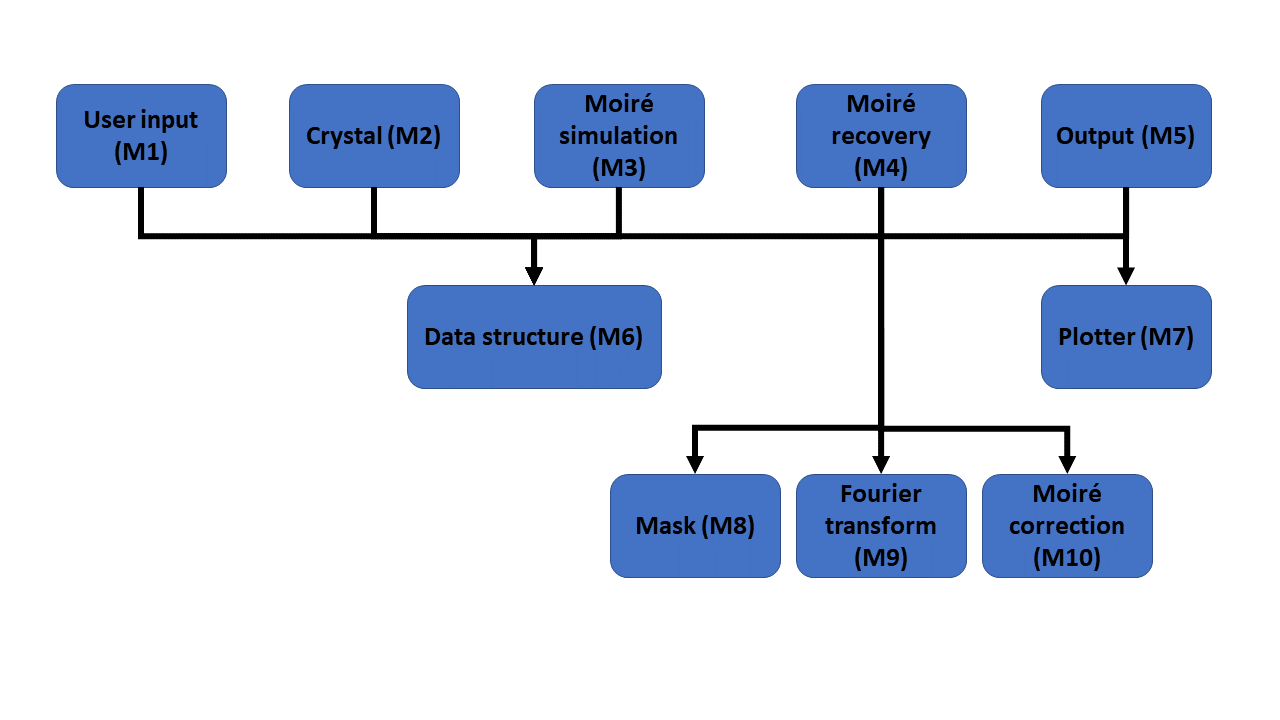
\includegraphics[width=\linewidth]{Figure_MG_STEMMoireRec.png}
\caption{Use hierarchy among modules}
\label{FigUH}
\end{figure}

\newpage

\bibliographystyle{ieeetr}
\bibliography{MG}

\end{document}
